{ %section3_6
	\subsection{Технология OpenCL}
	\label{OpenCL:section}
	\par\textbf{Краткая характеристика технологии.} OpenCL — фреймворк для написания компьютерных программ, связанных с параллельными вычислениями на различных графических и центральных процессорах, а также FPGA. В OpenCL входят язык программирования, который основан на стандарте языка программирования Си C99, и интерфейс программирования приложений. OpenCL обеспечивает параллелизм на уровне инструкций и на уровне данных и является осуществлением техники GPGPU. OpenCL является полностью открытым стандартом, его использование не облагается лицензионными отчислениями. С помощью этой технологии можно производить гетерогенные параллельные вычисления (распределять задачи между разными устройствами).
	\parКак мы уже знаем, можно распараллелить программу по задачам между небольшим числом производительных ядер (процессоры современных ПК) или по данным между тысячами простых медленных ядер (вычислительные ядра современных GPU). Именно для задач, решаемых с помощью распараллеливания по данным используется OpenCL.
	\par\textbf{Архитектура технологии OpenCL.} В OpenCL разделяют два вида устройств: \textit{host}, который управляет общей логикой и \textit{device}, которые выполняют вычисления. В роли \textit{хоста} обычно выступает центральный процессор, а в роли \textit{device} - GPU и другие устройства. \textit{Device} делится на вычислительные модули \textit{computer units}, которые в свою очередь состоят из обрабатывающих элементов (\textit{processing elements}) (рисунок~\ref{OpenCLArchitecture:image}). Непосредственно вычисления производятся в обрабатывающих элементах устройства.
	\begin{figure}[H]
		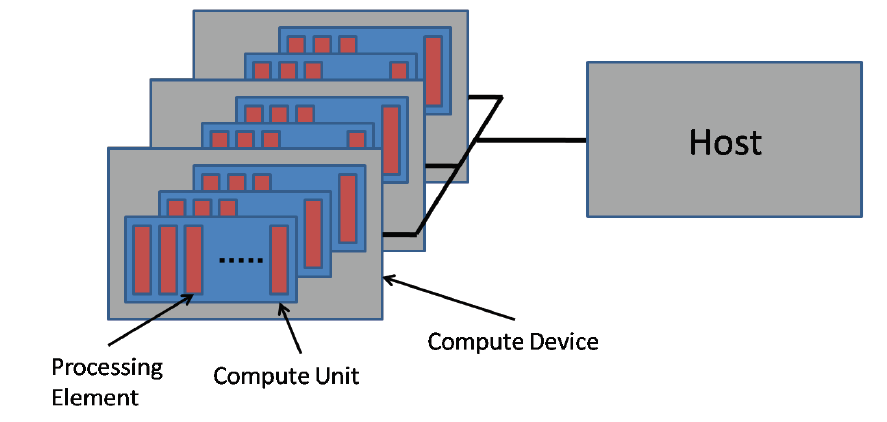
\includegraphics[width=1\linewidth]{OpenCLArchitecture}
		\caption{\textit{Архитектура OpenCL}}
		\label{OpenCLArchitecture:image}
	\end{figure}
	\parФизически \textit{computer unit} представляет собой \textit{work-group}, который состоит из ячеек \textit{work-item}, которые и выполняют вычисления (рисунок~\ref{OpenCLWorkGroup:image}).
	\begin{figure}[H]
		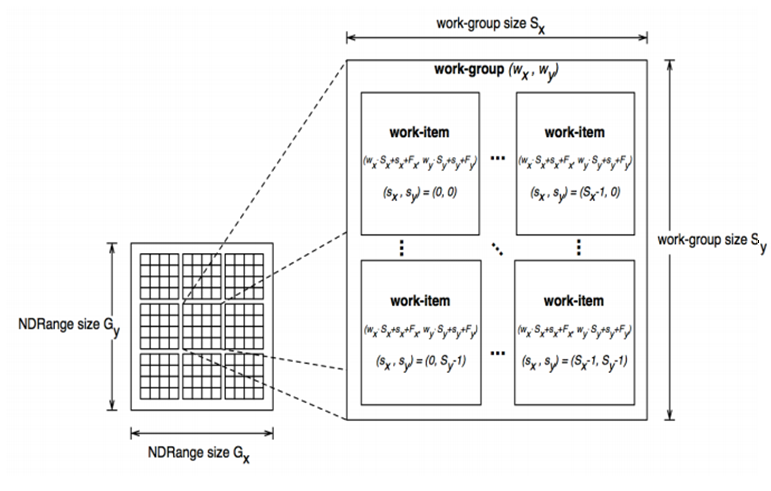
\includegraphics[width=1\linewidth]{OpenCLWorkGroup}
		\caption{\textit{Архитектура OpenCL - строение work-group элемента}}
		\label{OpenCLWorkGroup:image}
	\end{figure}
	\parКоманды в OpenCL, образуют очередь. \textit{Host} направляет команды на устройства. Эти команды становятся в очередь аналогичных команд. Можно реализовать очередь с соблюдением порядка и без соблюдения.
	Функции работы с получением ID \textit{work-group} и \textit{work-item} приведены на рисунке~\ref{OpenCLWorkGroupItemExample:image}.
	\begin{figure}[H]
		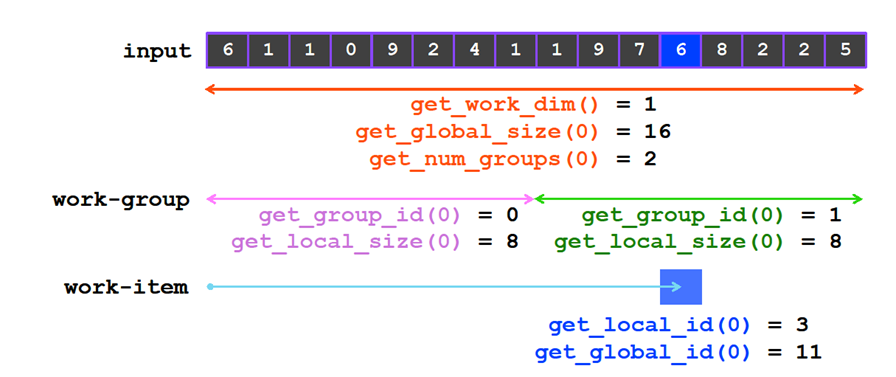
\includegraphics[width=1\linewidth]{OpenCLWorkGroupItemExample}
		\caption{\textit{OpenCL. Работа с work-group и work-item}}
		\label{OpenCLWorkGroupItemExample:image}
	\end{figure}
	\par\textbf{Виды памяти в OpenCL-устройствах.} Для взаимодействия с данными программист может использовать разные уровни памяти. На рисунке~\ref{OpenCLMemory:image} видно, что существуют следующие виды памяти:
	\begin{itemize}
		\itemЧастная память (private). Самая быстрая из всех видов. Эксклюзивна для каждого элемента работы.
		\itemЛокальная память (local memory). Может быть использована компилятором при большом количестве локальных переменных в какой-либо функции. По скоростным характеристикам локальная память значительно медленнее, чем регистровая. Доступ из элементов работе в одной work-group.
		\itemКонстантная память (constant memory). Достаточно быстрая из доступных GPU. Есть возможность записи данных с хоста, но при этом в пределах всего GPU возможно лишь чтение. Динамическое выделение в отличие от глобальной памяти в константной не поддерживается.
		\itemГлобальная память (global memory). Самый медленный тип памяти, из доступных GPU. Глобальные переменные можно выделить с помощью спецификатора, а также динамически. Глобальная память в основном служит для хранения больших объемов данных, поступивших на device с host’а. В алгоритмах, требующих высокой производительности, количество операций с глобальной памятью необходимо свести к минимуму.
	\end{itemize}	
	\begin{figure}[H]
		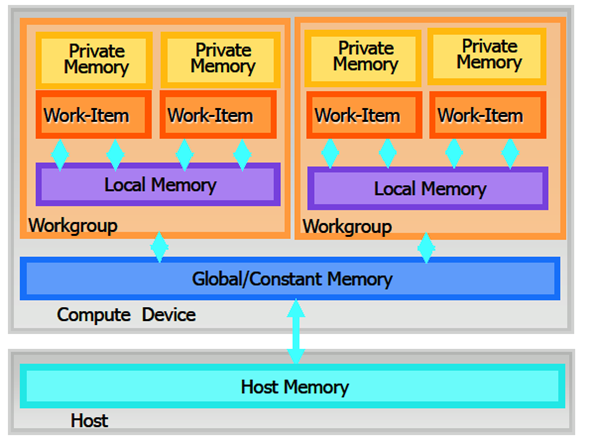
\includegraphics[width=1\linewidth]{OpenCLMemory}
		\caption{\textit{Виды памяти в OpenCL-устройствах}}
		\label{OpenCLMemory:image}
	\end{figure}
	Программист должен явно отдавать копирования между разной памятью.
	\parПрограмма на OpenCL может включать в себя следующую последовательность действий:
		\begin{enumerate}
			\item\textbf{Выбор платформы:} clGetPlatformIDs, clGetPlatformInfo
			\item\textbf{Выбор устройства:} clGetDeviceIDs, clGetDeviceInfo
			\item\textbf{Создание вычислительного контекста:} clCreateContextFromType
			\item\textbf{Создание очереди команд:} clCreateCommandQueueWithProperties
			\item\textbf{Выделение памяти в виде буферов:} clCreateBuffer
			\item\textbf{Создание объекта «программа»:} clCreateProgramWithSource
			\item\textbf{Компиляция кода:} clBuildProgram
			\item\textbf{Создание «ядра» (объект kernel):} clCreateKernel
			\item\textbf{Работа c Work-Group:} clGetKernelWorkGroupInfo 
			\item\textbf{Выполнение ядра:} clEnqueueNDRangeKernel 
			\item\textbf{Ожидание выполнения ядра:} clWaitForEvents 
			\item\textbf{Profiling:} clGetEventProfilingInfo
		\end{enumerate}
	Далее рассмотрим некоторые из этих действий подробнее.
	\par\textbf{Выбор платформы, устройства и создание контекста.} Контекст \textit{(context)} служит для управления объектами и ресурсами OpenCL. Все ресурсы OpenCL привязаны к контексту. С контекстом ассоциированы следующие данные (рисунок~\ref{OpenCLContext:image}):
		\begin{itemize}
			\itemустройства
			\itemобъекты программ
			\itemядра
			\itemобъекты памяти
			\itemочереди команд.
		\end{itemize}
	\begin{figure}[H]
		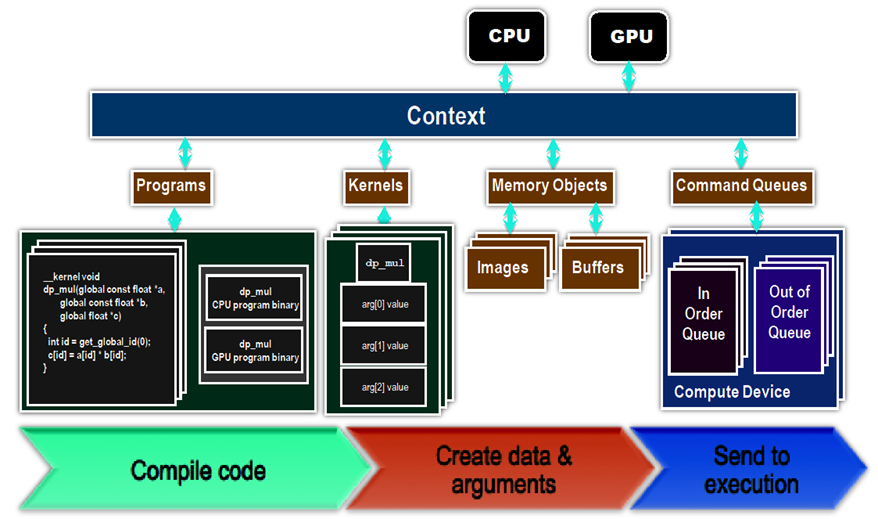
\includegraphics[width=1\linewidth]{OpenCLContext}
		\caption{\textit{Архитектура OpenCL - контекст}}
		\label{OpenCLContext:image}
	\end{figure}
	Можно получить информацию о платформе и вычислительных ядер с помощью специальных функций, чтобы затем создать контекст:
		\begin{itemize}
			\item\textit{clGetPlatformInfo()} - содержит информацию о платформе, на которой работает программа
			\item\textit{clGetDeviceDs()} - содержит информацию о подключенных устройствах
			\item\textit{clGetDeviceInfo()} - содержит информацию о данном девайсе: его тип, совместимость и тд.
		\end{itemize}
	Контекст можно создать при помощи функции \textit{clCreateContext()}. Вот пример его создания:
	\begin{figure}[H]
		\lstinputlisting{OpenCLContextExample.c}
	\end{figure}
	В строку 3 мы получаем ID платформы, в строке 7 ID первого GPU на этой платформе, в строке 11 создаем контекст для этого девайса. Подробнее про аргументы, принимаемые этими функциями можно прочитать в документации. Есть также функция \textit{clCreateContextFromType()} для создания контекста, ассоциированного с устройствами определенного типа.
	\par\textbf{Ядро.} Ядром называется функция, являющаяся частью программы и параллельно исполняющаяся на устройстве. Ядро является аналогом потоковой функции. Часть, выполняющаяся на устройстве, состоит из набора ядер, объявленных с квалификатором \textbf{\textunderscore \textunderscore kernel}. Компилирование ядер может осуществляться во время исполнения программы с помощью функций API. Работа в рамках одной work group выполняется одновременно всеми work items.
	\parПри написании ядра можно использовать следующие квалификаторы для переменнных:
		\begin{itemize}
			\item\textunderscore \textunderscore global или global – данные в глобальной памяти.
			\item\textunderscore \textunderscore constant или constant – данные в константной памяти.
			\item\textunderscore \textunderscore local или local – данные в локальной памяти.
			\item\textunderscore \textunderscore private или private – данные в частной памяти.
			\item\textunderscore \textunderscore read\textunderscore only и \textunderscore \textunderscore write\textunderscore only – квалификаторы режима доступа.
		\end{itemize}
	\parСкомпилировать код ядра можно с помощью функций \\ \textit{clCreateProgramWithSource()}, \textit{clBuildProgram()} и \textit{clCreateKernel()}. Пример компиляции и запуска программы по перемножению двух массивов приведен на рисунке~\ref{OpenCLKernelExample:image}.
	\begin{figure}[H]
		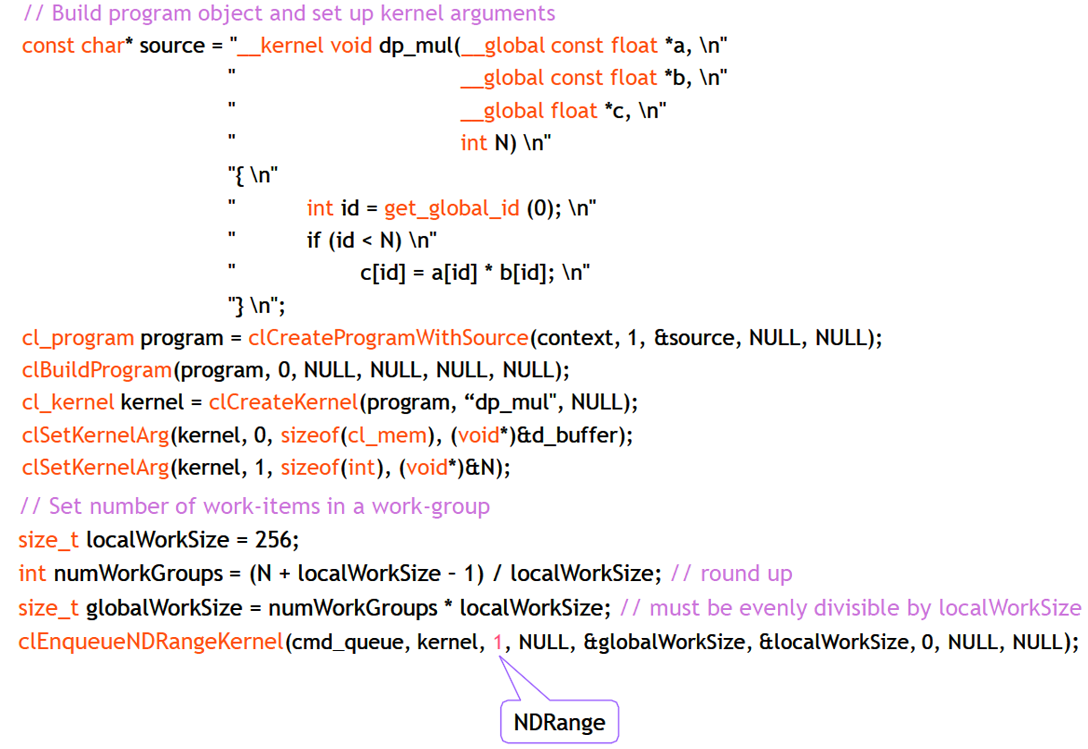
\includegraphics[width=1\linewidth]{OpenCLKernelExample}
		\caption{\textit{OpenCL - компиляция и запуск ядра}}
		\label{OpenCLKernelExample:image}
		%\lstinputlisting{OpenCLKernelExample.c}
	\end{figure}
	\sloppyПодробнее об остальных особенностях технологии OpenCL можно прочитать на ресурсе \url{http://docplayer.ru/37490743-Programmirovanie-na-opencl.html} и в официальной документации
	\begin{enumerate}
		\sloppy
		\item OpenCL – официальный сайт:\url{http://www.khronos.org/opencl/}
		\item Intel OpenCL: \url{http://software.intel.com/en-us/articles/intel-opencl-sdk/}
		\item NVIDIA OpenCL: \url{http://www.nvidia.ru/object/cuda\textunderscore opencl\textunderscore new\textunderscore ru.html}
		\item AMD OpenCL: \url{http://www.amd.com/us/products/technologies/stream-technology/opencl/Pages/opencl.aspx}
	\end{enumerate}
}